%* Source: https://tex.stackexchange.com/a/404849
\documentclass[tikz]{standalone}
\usepackage{pgfplots}
\pgfplotsset{compat=1.15}

\begin{document}
\footnotesize

    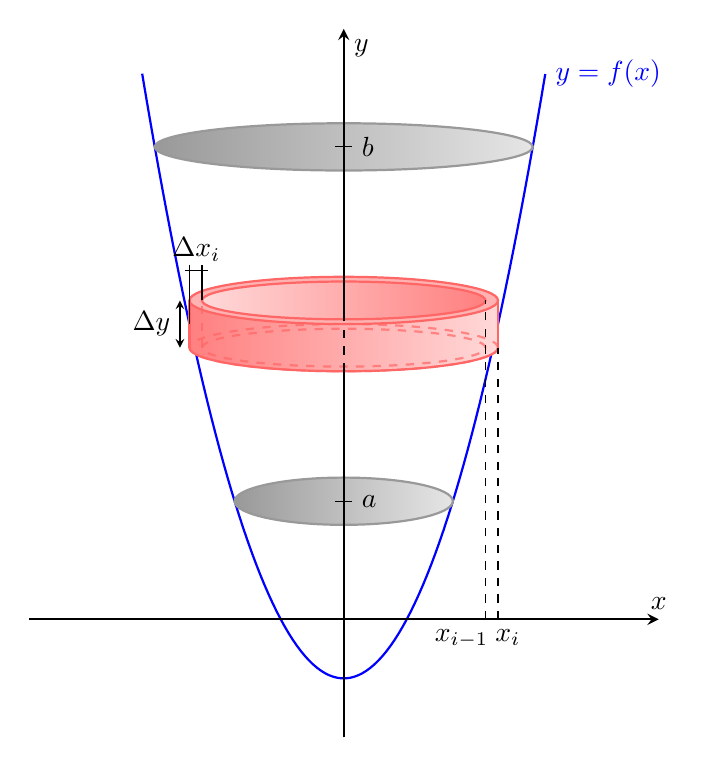
\begin{tikzpicture}[%
            scale=1,
            >=stealth,
            x=0.8cm,
            y=1.5cm,
            ]
    \tikzset{cyl/.style = {thick,color=red!60}}
    \tikzset{ellip/.style = {gray!80, shading=axis, top color=gray!80, right color=gray!20, thick}}

    %\fill[fill=green, opacity=0.4] (-3,4) -- plot[domain=-3:3](\x,{0.5*(\x*\x-1)}) -- (3,4);
    %\fill[fill=white] (-1.732050808,1) -- plot[domain=-1.732050808:1.732050808] (\x,{0.5*(\x*\x-1)}) -- (1.732050808,1); 

    % Parabola
    \draw[-, blue, thick, domain=-3.2:3.2, samples=100] plot (\x,{0.5*(\x*\x-1)}) node[right] {$y=f(x)$};

    % Ellipses & Cyllinder
    \shadedraw[ellip] (0,4) circle [y radius =.2, x radius =3];
    \shadedraw[ellip] (0,1) circle [y radius =.2, x radius =1.732050808];
    \shadedraw[cyl, shading=axis, top color=red!50, right color=red!15] (0,2.3) circle [y radius =.2, x radius =2.449489743];
    \shadedraw[cyl, draw=none, shading=axis, top color=red!50, right color=red!15] (-2.449489743,2.3) rectangle (2.449489743,2.7);
    \draw[cyl, fill=red!30] (0,2.7) circle [y radius =.2, x radius =2.449489743];
    \shadedraw[cyl, shading=axis, top color=red!15, right color=red!50] (0,2.7) circle [y radius =.16, x radius =2.25];
    \draw[cyl, opacity=0.7, dashed] (0,2.3) circle [y radius =.16, x radius =2.25];
    \draw[cyl, opacity=0.7, dashed] (0,2.3) circle [y radius =.2, x radius =2.449489743];
    \draw[dashed] (2.449489743,0) -- (2.449489743,2.7);
    \draw[dashed] (2.25,0) -- (2.25,2.7);
    \draw[cyl, opacity=0.7, dashed] (-2.25,2.3) -- (-2.25,2.7);
    \draw[cyl] (2.449489743,2.3) -- (2.449489743,2.7);
    \draw[cyl] (-2.449489743,2.3) -- (-2.449489743,2.7);

    % Dimensions
    \draw (-3pt,1) -- (3pt,1) node[right] {$a$};
    \draw (-3pt,4) -- (3pt,4) node[right] {$b$};
    \draw (-57.5pt,2.95) -- node[anchor=south] {\(\Delta x_i\)} (-49pt,2.95);
    \draw (-2.449489743,2.5) -- (-2.449489743,3);
    \draw (-2.25,2.7) -- (-2.25,3);
    \node at (2.25,0) [below right] {$x_i$};
    \node at (2.449489743,0) [below left] {$x_{i-1}$};
    \draw[<->, >=stealth] (-2.6,2.3) -- (-2.6,2.7) node[left, midway] {$\Delta y$};

    % Axes
    \draw[thick] (0,-1) -- (0,2.1);
    \draw[thick, dashed] (0,2.1) -- (0,2.535);
    \draw[->, thick] (0,2.535) -- (0,5) node[below right] {$y$};
    \draw[->, thick] (-5,0) -- (5,0) node[above] {$x$};

    \end{tikzpicture}
\end{document}